\documentclass[preprint,12pt,authoryear]{elsarticle}

\usepackage{amsmath}
\usepackage{amssymb}
\usepackage{booktabs}
\usepackage{CJKutf8}
\usepackage{graphicx}
\usepackage{hyperref}

\graphicspath{{../../../outputs/figures/}}
\biboptions{round,authoryear}
\hypersetup{hidelinks}
\journal{Research Process Report}

\begin{document}

\begin{frontmatter}

\title{Titanic Passenger Characteristics and Survival: A Research Process Report}

\begin{abstract}
\begin{CJK*}{UTF8}{gbsn}
\textbf{说明：}本文档是研究过程汇报，用于展示当前阶段的数据、方法、初步结果和下一步，不代表完整论文或最终研究结论。
\end{CJK*}

This process report examines how passenger sex, class, age, and family travel structure are associated with survival in the labelled Titanic competition data.

The current workflow audits the source files, constructs family variables, reports descriptive rates, estimates Logistic models, checks age-missing sensitivity and simple diagnostics, and evaluates lightweight internal prediction performance.

The estimates describe conditional associations in an observational historical dataset and do not identify causal effects or constitute a Kaggle ranking result.
\end{abstract}

\begin{keyword}
Titanic \sep survival \sep Logistic regression \sep missing data \sep reproducible analysis
\end{keyword}

\end{frontmatter}

\section{Research question}

The research question is how passenger sex, class, age, and family travel structure are associated with survival probability.

The unit of analysis is one passenger in the labelled training data.

The project deliberately excludes causal claims, leaderboard optimization, and prediction submission.

\section{Data source and use restrictions}

The data are the official \texttt{train.csv} and \texttt{test.csv} files from the Kaggle Titanic competition.

Access requires a Kaggle account, acceptance of the competition rules, and authenticated download.

The labelled file contains 891 passengers and is the sole basis for the association analysis and cross-validation.

The unlabelled file contains 418 passengers and is used only to confirm official acquisition and structural compatibility.

No prediction file was submitted to Kaggle.

\section{Sample and variables}

The outcome is the binary \texttt{Survived} field.

The focal variables are \texttt{Sex}, \texttt{Pclass}, \texttt{Age}, and family travel structure.

Family size is defined as \texttt{SibSp + Parch + 1}.

The descriptive workflow also distinguishes passengers travelling alone, small family groups of two to four, and large groups of five or more.

The adjusted model additionally includes log transformed fare and embarkation indicators because they have direct substantive interpretations in this dataset.

\section{Data quality and missingness}

The source audit confirmed the expected 12 training columns, 11 test columns, nonmissing unique passenger identifiers, no exact duplicate rows, compatible schemas, and allowed value ranges.

Age is missing for 177 training passengers, corresponding to 19.9\% of the labelled sample.

Cabin is missing for 687 training passengers and is excluded from the current model because its high missingness and coding require separate design work.

Embarkation is missing for two training passengers, while the unlabelled file has 86 missing ages, one missing fare, and 327 missing cabins.

The main association model replaces missing age with the training-sample median and includes an age-missing indicator.

A complete-age model using 714 passengers provides a direct missing-data sensitivity comparison.

\begin{table}[htbp]
\centering
\caption{Descriptive statistics for the Titanic analysis sample.}
\label{tab:descriptive}
\small
\resizebox{\linewidth}{!}{%
\begin{tabular}{lrrrrrrrrr}
\toprule
Variable & N & Missing & Mean & SD & Median & Q1 & Q3 & Min & Max \\
\midrule
Survived & 891 & 0 & 0.38 & 0.49 & 0.00 & 0.00 & 1.00 & 0.00 & 1.00 \\
Age & 714 & 177 & 29.70 & 14.53 & 28.00 & 20.12 & 38.00 & 0.42 & 80.00 \\
Fare & 891 & 0 & 32.20 & 49.69 & 14.45 & 7.91 & 31.00 & 0.00 & 512.33 \\
FamilySize & 891 & 0 & 1.90 & 1.61 & 1.00 & 1.00 & 2.00 & 1.00 & 11.00 \\
\bottomrule
\end{tabular}
}
\end{table}


\section{Descriptive analysis}

Overall survival in the labelled sample is 38.4\%.

Observed survival is 74.2\% among women and 18.9\% among men.

Observed survival is 63.0\%, 47.3\%, and 24.2\% in first, second, and third class respectively.

Small family groups have 57.9\% observed survival, compared with 30.4\% among passengers travelling alone and 16.1\% among groups of five or more.

Figure~\ref{fig:group-rates} shows these descriptive rates with Wilson intervals and should not be read as an adjusted or causal comparison.

\begin{figure}[htbp]
\centering
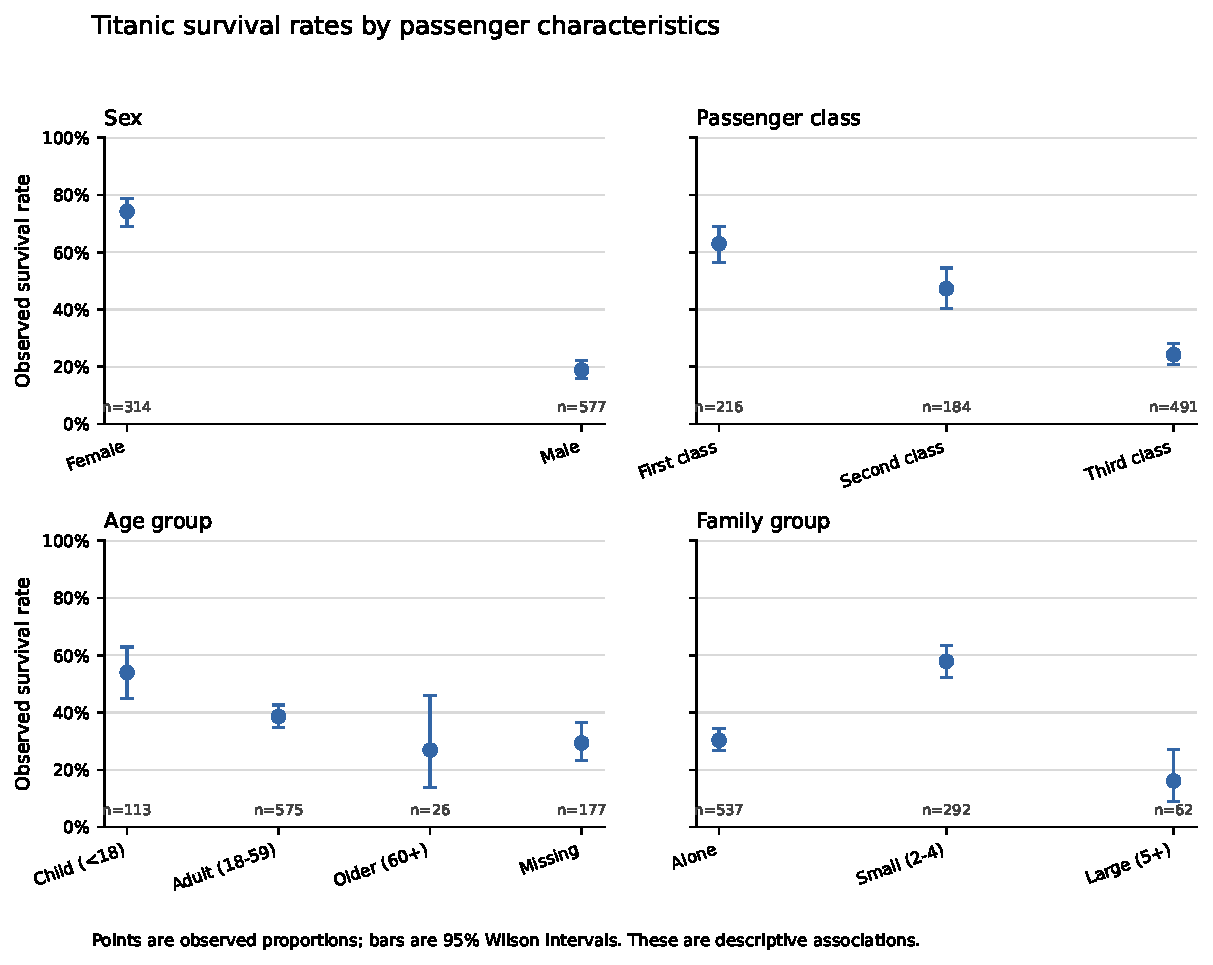
\includegraphics[width=\textwidth]{survival-rates-by-characteristics.pdf}
\caption{Observed survival rates by passenger sex, class, age group, and family group with 95\% Wilson intervals.}
\label{fig:group-rates}
\end{figure}

\section{Logistic regression method}

The main Logistic model includes sex, class indicators, age per ten years, family size, log fare, embarkation indicators, and the age-missing indicator.

Male passengers, third class, and embarkation at Southampton are the categorical reference levels.

The model reports log-odds coefficients, standard errors, two-sided Wald tests, odds ratios, and 95\% confidence intervals.

The complete-age sensitivity model uses the same shared terms but omits the missing-age indicator.

The model is descriptive and does not resolve unobserved confounding, selection, measurement error, or historical mechanisms that generated the recorded variables.

\section{Preliminary association results}

After adjustment for the other model variables, the female versus male odds ratio is 14.89 with a 95\% confidence interval from 10.03 to 22.08.

The first versus third class odds ratio is 5.54 with a 95\% confidence interval from 2.72 to 11.29.

The second versus third class odds ratio is 2.82 with a 95\% confidence interval from 1.72 to 4.61.

The odds ratio for each additional ten years of age is 0.68 with a 95\% confidence interval from 0.58 to 0.79.

The odds ratio for each additional family passenger is 0.74 with a 95\% confidence interval from 0.63 to 0.86.

The complete-age sensitivity model preserves the directions of the focal terms, although the first-class estimate rises from 5.54 to 9.07 and several secondary adjustment intervals remain wide.

Figure~\ref{fig:odds-ratios} and Table~\ref{tab:logit-main} report the main adjusted associations.

\begin{figure}[htbp]
\centering
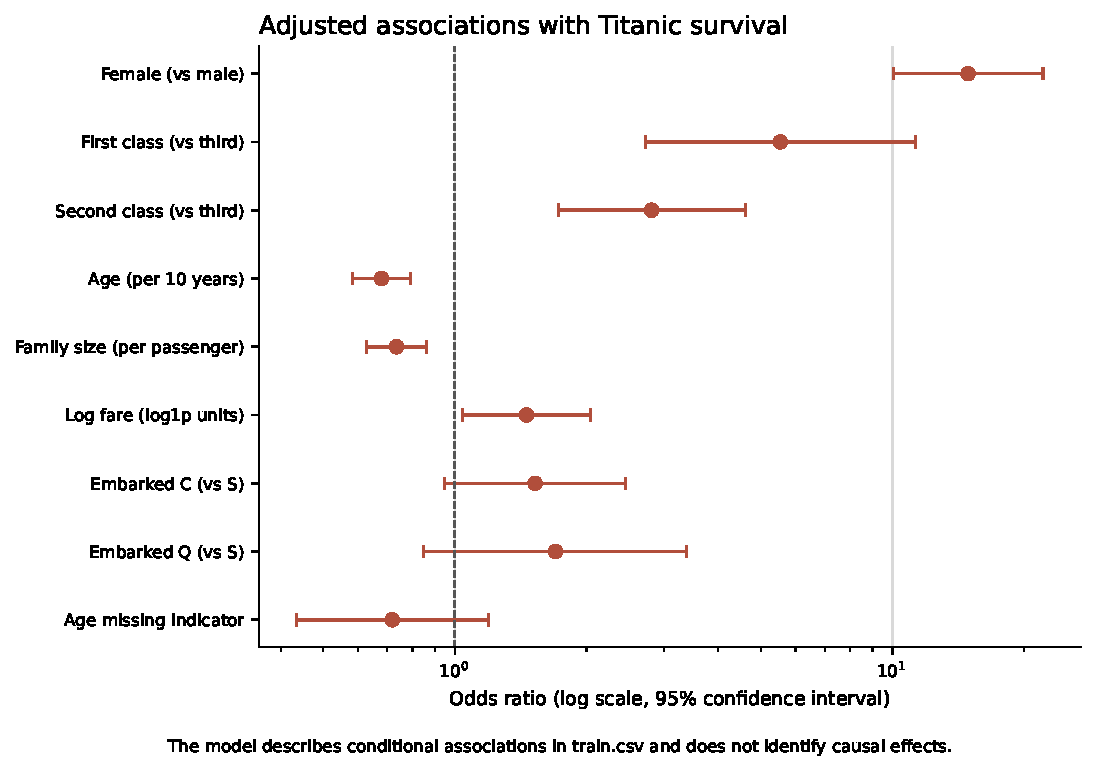
\includegraphics[width=\textwidth]{main-model-odds-ratios.pdf}
\caption{Main-model odds ratios and 95\% confidence intervals on a logarithmic scale.}
\label{fig:odds-ratios}
\end{figure}

\begin{table}[htbp]
\centering
\caption{Main Logistic regression associations with survival.}
\label{tab:logit-main}
\small
\begin{tabular}{lrrr}
\toprule
Term & Odds ratio & 95\% CI & p-value \\
\midrule
Female (vs male) & 14.89 & 10.03--22.08 & <0.001 \\
First class (vs third) & 5.54 & 2.72--11.29 & <0.001 \\
Second class (vs third) & 2.82 & 1.72--4.61 & <0.001 \\
Age (per 10 years) & 0.68 & 0.58--0.79 & <0.001 \\
Family size (per passenger) & 0.74 & 0.63--0.86 & <0.001 \\
Log fare (log1p units) & 1.46 & 1.04--2.04 & 0.028 \\
Embarked C (vs S) & 1.52 & 0.95--2.45 & 0.082 \\
Embarked Q (vs S) & 1.70 & 0.85--3.39 & 0.134 \\
Age missing indicator & 0.72 & 0.43--1.19 & 0.200 \\
\bottomrule
\end{tabular}
\end{table}


\section{Diagnostics and internal prediction performance}

All variance inflation factors are below 3 in the main design, providing no simple indication of severe linear collinearity.

Fifty-four passengers exceed the exploratory Cook distance threshold of four divided by the sample size.

These observations are retained, and the threshold is treated as a prompt for influence review rather than an automatic deletion rule.

Five-fold stratified cross-validation uses random seed 20260810 and performs age imputation inside each training fold.

The out-of-fold ROC AUC is 0.851 and the Brier score is 0.144.

The out-of-fold calibration intercept is -0.013 and the slope is 0.996 in this same internal sample.

These metrics are lightweight internal checks and are not evidence of external validity or competition standing.

\begin{table}[htbp]
\centering
\caption{Five-fold stratified cross-validation performance within train.csv.}
\label{tab:model-performance}
\small
\begin{tabular}{lrrrrr}
\toprule
Metric & OOF & Fold mean & Fold SD & Folds & Seed \\
\midrule
ROC AUC & 0.851 & 0.853 & 0.019 & 5 & 20260810 \\
Brier score & 0.144 & 0.144 & 0.012 & 5 & 20260810 \\
Log loss & 0.451 & 0.451 & 0.030 & 5 & 20260810 \\
\bottomrule
\end{tabular}
\end{table}


\section{Limitations}

The data are observational and historically specific, so the associations do not identify causal effects.

The available variables do not capture all social, spatial, operational, and recording processes related to survival.

Median age imputation is transparent but does not model the missing-data mechanism or propagate imputation uncertainty.

The current continuous age and family-size terms impose functional-form assumptions that may hide nonlinear patterns.

The Cook distance screen identifies a nontrivial set of potentially influential observations that still requires case-level examination.

Cross-validation is internal to one small labelled dataset, and the unlabelled official test file cannot provide an outcome-based validation.

\section{Next steps}

The next analysis step is to inspect influential observations without deleting them solely because they cross a heuristic threshold.

A prespecified comparison can test nonlinear age and family-size specifications while retaining the current model as the reference.

If the project moves beyond this demonstration, a later analysis can use multiple imputation for missing ages.

External validation requires a separate labelled dataset with documented provenance and compatible variables.

The process report should be revised only when those analyses create new evidence, and no Kaggle submission is planned.

\end{document}
